%%%%%%%%%%%%%%%%%%%%%%%%%%%%%%%%%%%%%%%%%%%%%%%%%%%%%%%%%%%%%%%%%%%%%%%%%%%%%%%%%%%%%%%%%%%%%%%%%%%%%%%%%%%%%%%%%%%%%%%%%%%%%%%%%%%%%%%%%%%%%%%%%%%%%%%%%%%
% This is just an example/guide for you to refer to when submitting manuscripts to Frontiers, it is not mandatory to use Frontiers .cls files nor frontiers.tex  %
% This will only generate the Manuscript, the final article will be typeset by Frontiers after acceptance.                                                 %
%                                                                                                                                                         %
% When submitting your files, remember to upload this *tex file, the pdf generated with it, the *bib file (if bibliography is not within the *tex) and all the figures.
%%%%%%%%%%%%%%%%%%%%%%%%%%%%%%%%%%%%%%%%%%%%%%%%%%%%%%%%%%%%%%%%%%%%%%%%%%%%%%%%%%%%%%%%%%%%%%%%%%%%%%%%%%%%%%%%%%%%%%%%%%%%%%%%%%%%%%%%%%%%%%%%%%%%%%%%%%%

%%% Version 3.1 Generated 2015/22/05 %%%
%%% You will need to have the following packages installed: datetime, fmtcount, etoolbox, fcprefix, which are normally inlcuded in WinEdt. %%%
%%% In http://www.ctan.org/ you can find the packages and how to install them, if necessary. %%%

\documentclass{frontiersSCNS} % for Science, Engineering and Humanities and Social Sciences articles
%\documentclass{frontiersHLTH} % for Health articles
%\documentclass{frontiersFPHY} % for Physics and Applied Mathematics and Statistics articles

%\setcitestyle{square}
\usepackage{url,hyperref,lineno,microtype}
\usepackage[onehalfspacing]{setspace}
\usepackage{graphicx}
\usepackage{caption}
\usepackage{subcaption}
\graphicspath{ {images/} }
\linenumbers



\makeatletter
\let\save@mathaccent\mathaccent
\newcommand*\if@single[3]{%
  \setbox0\hbox{${\mathaccent"0362{#1}}^H$}%
  \setbox2\hbox{${\mathaccent"0362{\kern0pt#1}}^H$}%
  \ifdim\ht0=\ht2 #3\else #2\fi
  }
%The bar will be moved to the right by a half of \macc@kerna, which is computed by amsmath:
\newcommand*\rel@kern[1]{\kern#1\dimexpr\macc@kerna}
%If there's a superscript following the bar, then no negative kern may follow the bar;
%an additional {} makes sure that the superscript is high enough in this case:
\newcommand*\widebar[1]{\@ifnextchar^{{\wide@bar{#1}{0}}}{\wide@bar{#1}{1}}}
%Use a separate algorithm for single symbols:
\newcommand*\wide@bar[2]{\if@single{#1}{\wide@bar@{#1}{#2}{1}}{\wide@bar@{#1}{#2}{2}}}
\newcommand*\wide@bar@[3]{%
  \begingroup
  \def\mathaccent##1##2{%
%Enable nesting of accents:
    \let\mathaccent\save@mathaccent
%If there's more than a single symbol, use the first character instead (see below):
    \if#32 \let\macc@nucleus\first@char \fi
%Determine the italic correction:
    \setbox\z@\hbox{$\macc@style{\macc@nucleus}_{}$}%
    \setbox\tw@\hbox{$\macc@style{\macc@nucleus}{}_{}$}%
    \dimen@\wd\tw@
    \advance\dimen@-\wd\z@
%Now \dimen@ is the italic correction of the symbol.
    \divide\dimen@ 3
    \@tempdima\wd\tw@
    \advance\@tempdima-\scriptspace
%Now \@tempdima is the width of the symbol.
    \divide\@tempdima 10
    \advance\dimen@-\@tempdima
%Now \dimen@ = (italic correction / 3) - (Breite / 10)
    \ifdim\dimen@>\z@ \dimen@0pt\fi
%The bar will be shortened in the case \dimen@<0 !
    \rel@kern{0.6}\kern-\dimen@
    \if#31
      \overline{\rel@kern{-0.6}\kern\dimen@\macc@nucleus\rel@kern{0.4}\kern\dimen@}%
      \advance\dimen@0.4\dimexpr\macc@kerna
%Place the combined final kern (-\dimen@) if it is >0 or if a superscript follows:
      \let\final@kern#2%
      \ifdim\dimen@<\z@ \let\final@kern1\fi
      \if\final@kern1 \kern-\dimen@\fi
    \else
      \overline{\rel@kern{-0.6}\kern\dimen@#1}%
    \fi
  }%
  \macc@depth\@ne
  \let\math@bgroup\@empty \let\math@egroup\macc@set@skewchar
  \mathsurround\z@ \frozen@everymath{\mathgroup\macc@group\relax}%
  \macc@set@skewchar\relax
  \let\mathaccentV\macc@nested@a
%The following initialises \macc@kerna and calls \mathaccent:
  \if#31
    \macc@nested@a\relax111{#1}%
  \else
%If the argument consists of more than one symbol, and if the first token is
%a letter, use that letter for the computations:
    \def\gobble@till@marker##1\endmarker{}%
    \futurelet\first@char\gobble@till@marker#1\endmarker
    \ifcat\noexpand\first@char A\else
      \def\first@char{}%
    \fi
    \macc@nested@a\relax111{\first@char}%
  \fi
  \endgroup
}
\makeatother

% Leave a blank line between paragraphs instead of using \\


\def\keyFont{\fontsize{8}{11}\helveticabold }
\def\firstAuthorLast{Giavasis {et~al.}} %use et al only if is more than 1 author

\def\Authors{Steven Giavasis\,$^{1,2}$,
        Sang Han Lee\,$^{2}$,
        Zarrar Shehzad\,$^{1,2,3}$,
        Qingyang Li\,$^{1}$,
        Yassine Benhajali\,$^{4,5}$,
        Chaogan Yan\,$^{6}$,
        Zhen Yang\,$^{7}$,
        Michael Milham\,$^{1,8}$,
        Pierre Bellec\,$^{5}$,
        R. Cameron Craddock\,$^{1,2,*}$
}


% Affiliations should be keyed to the author's name with superscript numbers and be listed as follows: Laboratory, Institute, Department, Organization, City, State abbreviation (USA, Canada, Australia), and Country (without detailed address information such as city zip codes or street names).
% If one of the authors has a change of address, list the new address below the correspondence details using a superscript symbol and use the same symbol to indicate the author in the author list.
\def\Address{$^{1}$Center for the Developing Brain, Child Mind Institute, New York, NY, USA \\
             $^{2}$Computational Neuroimaging Laboratory, Center for Biomedical Imaging and Neuromodulation, Nathan S. Kline Institute for Psychiatric Research, Orangeburg, NY, USA \\
			 $^{3}$Department of Psychology, Yale University, New Haven, CT, USA \\
			 $^{4}$D\'{e}partement d'anthropologie, Universit\'{e} de Montr\'{e}al, Montr\'{e}al, QC, Canada \\
			 $^{5}$Centre de recherche de l’institut de g\'{e}riatrie de Montr\'{e}al, Montr\'{e}al, QC, Canada \\
			 $^{6}$Institute of Psychology, Chinese Academy of Science, Beijing, China \\
			 $^{7}$Department of Psychiatry, University of Pennsylvania Perelman School of Medicine, Philadelphia, PA, USA \\
			 $^{8}$Center for Biomedical Imaging and Neuromodulation, Nathan S. Kline Institute for Psychiatric Research, Orangeburg, NY, USA}



% The Corresponding Author should be marked with an asterisk
% Provide the exact contact address (this time including street name and city zip code) and email of the corresponding author
\def\corrAuthor{R. Cameron Craddock}
\def\corrAddress{Computational Neuroimaging Laboratory, Center for Biomedical Imaging and Neuromodulation, Nathan S. Kline Institute for Psychiatric Research, 140 Old Orangeburg Road, Orangeburg, NY, 10962, USA}\def\corrEmail{ccraddock@nki.rfmh.org}




\begin{document}
\onecolumn
\firstpage{1}

\title[Running Title]{The Preprocessed Connectomes Project Quality Assessment Protocol: a resource for measuring the quality of MRI data.} 

\author[\firstAuthorLast ]{\Authors} %This field will be automatically populated
\address{} %This field will be automatically populated
\correspondance{} %This field will be automatically populated

\extraAuth{}% If there are more than 1 corresponding author, comment this line and uncomment the next one.
%\extraAuth{corresponding Author2 \\ Laboratory X2, Institute X2, Department X2, Organization X2, Street X2, City X2 , State XX2 (only USA, Canada and Australia), Zip Code2, X2 Country X2, email2@uni2.edu}


\maketitle

%%%%%%%%%%%%%%%%%%%%%%%%%%%%%%%%%%%%%%%%%%%%%%%%%%%%%%%%%%%%%%%%%%%%%%%%%%%%%%%%%%%%%%%%%%%%%%%%%%%%%%%%%%%%%%%%%%%%%%%%%%%%%%%%%%%%%%%%%%%%%%%%%%%%%%%%%%%%%%%%%%%%%%%%%%%%%%%%%%%%%%%%%%%%%%%%%%%%%%%%%%%%%%%%%%%%%%%%%%%%%%%%%%%%%%%
%%% The sections below are for reference only.
%%%
%%% For Original Research Articles, Clinical Trial Articles, and Technology Reports the section headings should be those appropriate for your field and the research itself. It is recommended to organize your manuscript in the
%%% following sections or their equivalents for your field:
%%% Abstract, Introduction, Material and Methods, Results, and Discussion.
%%% Please note that the Material and Methods section can be placed in any of the following ways: before Results, before Discussion or after Discussion.
%%%
%%%For information about Clinical Trial Registration, please go to http://www.frontiersin.org/about/AuthorGuidelines#ClinicalTrialRegistration
%%%
%%% For Clinical Case Studies the following sections are mandatory: Abstract, Introduction, Background, Discussion, and Concluding Remarks.
%%%
%%% For all other article types there are no mandatory sections.
%%%%%%%%%%%%%%%%%%%%%%%%%%%%%%%%%%%%%%%%%%%%%%%%%%%%%%%%%%%%%%%%%%%%%%%%%%%%%%%%%%%%%%%%%%%%%%%%%%%%%%%%%%%%%%%%%%%%%%%%%%%%%%%%%%%%%%%%%%%%%%%%%%%%%%%%%%%%%%%%%%%%%%%%%%%%%%%%%%%%%%%%%%%%%%%%%%%%%%%%%%%%%%%%%%%%%%%%%%%%%%%%%%%%%%%

\begin{abstract}

%%% Leave the Abstract empty if your article falls under any of the following categories: Editorial Book Review, Commentary, Field Grand Challenge, Opinion or specialty Grand Challenge.
\section{}
%As a primary goal, the abstract should render the general significance and conceptual advance of the work clearly accessible to a broad readership. References should not be cited in the abstract.
For full guidelines regarding your manuscript please refer to \href{http://www.frontiersin.org/about/AuthorGuidelines}{Author Guidelines} \\ or \textbf{Table \ref{Tab:01}} for a summary according to article type.


\tiny
 \keyFont{ \section{Keywords:} Text Text Text Text Text Text Text Text } %All article types: you may provide up to 8 keywords; at least 5 are mandatory.
\end{abstract}

\section{Introduction}
\label{intro}
It is well accepted that poor quality data interferes with the ability of neuroimaging analyses to uncover biological signal and distinguish meaningful from artifactual findings, but there is no clear guidance on how to differentiate “good” from “bad” data. A variety of different measures have been proposed, but there is no evidence supporting the primacy of one measure over another or on the ranges of values for differentiating “good” from “bad” data. As a result, researchers are required to rely on painstaking visual inspection to assess data quality. But this approach consumes a lot of time and resources, is subjective, and is susceptible to inter-­rater and test-­retest variability. Additionally, it is possible that some defects are too subtle to be fully appreciated by visual inspection, yet are strong enough to degrade the accuracy of data processing algorithms or bias analysis results. Further, it is difficult to visually assess the quality of data that has already been processed, such as that being shared through the Preprocessed Connectomes Project (PCP; http://preprocessed­connectomes­project.github.io/), the Human Connectome Project (HCP), and the Addiction Connectomes Preprocessing Iniatiative (ACPI). To begin to address this problem, the PCP has assembled several of the quality metrics proposed in the literature to implement a Quality Assessment Protocol (QAP; http://preprocessed­connectomes­project.github.io/quality­assessment­protocol).

The QAP is a open source software package implemented in python for the automated calculation of quality measures for functional and structural MRI data. The QAP software makes use of the Nipype (\cite{gorgolewski2011}) pipelining library to efficiently acheive high throughput processing on a variety of different high performance computing systems. The quality of structural MRI data is assessed using contrast-­to-­noise ratio (CNR; \cite{magnotta2006}), entropy focus criterion (EFC, \cite{atkinson1997}), foreground-­to-­background energy ratio (FBER, ), voxel smoothness (FWHM, \cite{friedman2008}), percentage of artifact voxels (QI1, \cite{mortamet2009}), and signal­-to-­noise ratio (SNR, \cite{magnotta2006}). The QAP includes methods to assess both the spatial and temporal quality of fMRI data. Spatial quality is assessed using EFC, FBER, and FWHM, in addition to ghost-­to-­signal ratio (GSR). Temporal quality of functional data is assessed using the standardized root mean squared change in fMRI signal between volumes (DVARS; Nichols 2013), mean root mean square deviation (MeanFD, \cite{jenkinson2002}), the percentage of voxels with MeanFD $>$ 0.2 (Percent FD; \cite{power2012}), the temporal mean of AFNI’s 3dTqual metric (1 minus the Spearman correlation between each fMRI volume and the median volume; \cite{cox1996}), global correlation (the average correlation of every voxel in the timeseries with each other; \cite{saad2013}), and the average fraction of outliers found in each volume using AFNI’s 3dTout command.

Applying the QAP for differentiating good quality data from poor will require learning which of the measures are the most sensitive to problems in the data and the ranges of values for the measures that indicate poor data. The solutions to these questions are likely to vary based on the analyses at hand and finding them will likely require the ready availability of large scale hetereogenous datasets for which the QAP metrics have been calculated. To help with this goal, the QAP has been used to measure structural and temporal data quality on data from the Autism Brain Imaging Data Exchange (ABIDE; \cite{dimartino2014}) and the Consortium for Reliability and Reproducibility (CoRR, \cite{zuo2014}) and the results are being openly shared through the PCP. An initial analyses of the resulting values has been performed to evaluate their collinearity, correspondence to expert­-assigned quality labels, and test­-retest reliability.
\section{Methods}
\label{sec:1}
The Preprocessed Connectome’s Project Quality Assessment Protocol is an open source toolkit of quality assessment measures implemented in python. Calculating the measures requires several standard preprocessing procedures such as tissue segmentation, image registration and mask generation that are accomplished using components from FSL(;) and AFNI. These tools are integrated with QAP specific python functions using the Nipype pipelining library to automate processing of very large datasets in parallel on high performance computing systems such as multicore workstations and clusters that use Sun Grid Engine. The toolkit provides everything necessary to calculate the measures from scratch using raw imaging data but can also import data intermediaries (i.e. tissue segmentation maps) processed outside of the QAP pipeline. The software requires the images to be in the NIfTI file format and can handle a variety of different directory structures using an easy to construct configuration file. The software can be installed using standard python package installation tools (e.g. pip) and is available preinstalled on a free-to-use Amazon Machine Instance. Extensive documentation on installing and using the toolkit are available at its webpage ().
\section{The Metrics}
\label{sec:2}
The toobox includes a variety of different metrics for assessing spatial and temporal quality of data that have been proposed in the literature. The goal has been to make the toolbox comprehensive even though many of the measures may be highly correlated. Measures, such as signal-to-noise-fluctuation ratio (also known as temporal signal to noise ratio), that are only appropriate for phantom studies and have been excluded along with measures, such as QI2, that are overly complicated or computationally expensive with marginal sensitivity to quality (). When possible the amount of processing required for calculating the images has been minimized so that the measure focuses on the quality of the data rather than the quality of the algorithms used to perform the processing. But since some processing, such as segmentation, alignment, and masking, is unavoidable we recommend that QA measures be calculated using the same algorithms. QAP’s current version only includes measures for structural and functional MRI data, measures for other imaging modalities such as diffusion MRI will be added in the future.
\subsection{Measures of spatial quality}
\label{sec:3}
\subsubsection{Contrast-to-Noise Ratio (CNR)}
\label{sec:4}
CNR can be defined in many different ways depending on the purpose of the images being collected. Since structural MRI data is most commonly used for morphometric measurements and calculating tissue specific maps for downstream processing, the QAP focuses on the contrast between white matter and grey matter. CNR should correlate with how well anatomical features can be discerned from the image and provides a measure of how easily the image can be segmented. It is sensitive to the imaging parameters used to acquire the data, as well as, the amount of thermal noise, artifacts, and head motion present in the image. Higher values for CNR are better. CNR is only calcuated for structural MRI data.
\begin{equation}
CNR = \frac{\widebar{WM} - \widebar{GM}} {\sigma_{b}}
\end{equation}
CNR is the difference between the mean white matter signal and the mean gray matter signal divided by the standard deviation of the image background (Eqn. 1). The input structural MRI image is segmented into grey matter and white matter masks using FSL’s FAST. Image background is defined by inverting a whole head mask that was defined by sequentially dilating and eroding the result of AFNI’s 3dAutomask 4 times. The resulting GM and WM masks are applied to the input image to calculate the mean voxel intensity within each comparment, and the background mask is used to calculate the standard deviations of voxels outside of the head. 
\subsubsection{Entropy Focus Criterion (EFC)}
\label{sec:5}
EFC is calculated as the Shannon entropy of the voxel intensities. This value reaches its maximum when the number of voxels in the image are spread evenly over the different voxel intensities present in the image and will reach its minimum if the voxels are disproportionately focused on a single intensity value.
\begin{equation}
EFC = - \sum_{j=1}^{S} \frac{B_j}{B_{max}} \ln{\frac{B_j}{B_{max}}} \\
\end{equation}
with S being the number of image voxels, and B\_j being the voxel intensity. If all of the intensity in the image were concentrated in one voxel, the largest amount of intensity, B\_max, would be given by \\
\begin{equation}
B_{max} = \sqrt{\sum_{j=1}^{S} B_{j}^{2}}
\end{equation}
Since the majority of voxels in a structural brain image should have zero intensity, which are typically viewed as black, this measure is often interpreted as the “blackness” of the image. Ghosting and head motion should reduce the amount of black in the image background, and hence should increase EFC (Atkinson 1997). The lower this number is, the better. \\
\subsubsection{Foreground-to-Background Energy Ratio (FBER)}
\label{sec:6}
FBER is calculated by dividing the energy (normalized variance) of the image foreground by the energy of the background. In an ideal brain image all of the image energy should be contained in the foreground. Head motion, thermal noise, ghosting, and other artifacts will increase the energy in the images background and will reduce this value. Calculating FBER requires a head mask which is constructed by iterative dilating and eroding the output of 3dAutomask 4 times, background is defined as the inversion of this mask. Higher values of FBER are better. 
\subsubsection{Full-Width Half Maximum (FWHM)}
\label{sec:7}
This spatial metric measures how “smoothed” the image is, which is essentially a measure of the degree of spatial correlation in the image data. The QAP pipeline uses the AFNI command 3dFWHMx to calculate this value. The lower this number is, the better.
\subsubsection{Artifact Detection (Qi1)}
\label{sec:8}
For this measure, the proportion of voxels with intensity corrupted by artifacts is normalized by the number of voxels in the background (the air). The lower this number is, the better.
\subsubsection{Signal-to-Noise Ratio (SNR)}
\label{sec:9}
Given the anatomical segmentation maps and the anatomical head mask, the mean of the gray matter signal is calculated and then divided by the standard deviation of the mean of the signal values within the background (air). The higher this number is, the better.
\\\\
Like the spatial measures for anatomical data, the spatial quality measures for functional data include EFC, FBER, FWHM, and SNR. Unlike the spatial measures for anatomical data, however, these measures are run on the mean of the functional timeseries, which preserves the spatial features of the functional timeseries data. As mentioned above, in addition to these measures, there is another metric exclusive to the functional spatial metrics:
\subsubsection{Ghost-to-Signal Ratio (GSR)}
\label{sec:10}
The GSR is the mean of the signal in the “ghost” of the image (artifacts appearing outside of the brain, caused by phase discontinuities in the phase-encoding direction) relative to the mean signal within the brain. The user must know the phase-encoding direction related to the scans being analyzed. The lower this number is, the better.
\subsection{Measures of temporal quality}
\label{sec:11}
\subsubsection{Standardized DVARS}
\label{sec:12}
This measure is calculated by normalizing the spatial standard deviation of the temporal derivative of the data with the temporal standard deviation and temporal autocorrelation. The standardization, calculated by a script by Nichols [cite], provides a more absolute measure of DVARS which can be compared across subjects:
\begin{equation}
DVARS = {\frac{\sqrt{\frac{1}{I} \sum_{i} (Y_{i,t} - Y_{i,t - 1})^2}}{\sqrt{\frac{1}{I} \sum_{i} 2(1 - \rho_{i})\sigma_{i}^2}}
\end{equation}
Y\_i,t being fMRI time series data, i being voxels and t being time points. The lower this value is, the better.
\subsubsection{Outlier Detection}
\label{sec:13}
The AFNI tool 3dTout is used to find the mean fraction of outliers in each volume of the timeseries. The lower this value is, the better.
\subsubsection{Global Correlation (GCOR)}
\label{sec:14}
The global correlation measure is the average correlation of every combination of voxels in the functional time series. The difference in GCOR between time series can help identify differences in the data that arise from motion or physiological noise.
\subsubsection{Median Distance Index (Quality)}
\label{sec:15}
The AFNI tool 3dTqual is used to calculate a quality index describing the functional timeseries. This tool finds the volume of median value and then calculates the mean distance (Spearman’s rho) between each volume and the median. The lower this value is, the better.
\subsubsection{Mean Framewise Displacement (Jenkinson’s Mean FD)}
\label{sec:16}
A measure of subject head motion, which compares the motion between the current and previous volumes. This is calculated by summing the absolute value of displacement changes in the x, y and z directions and rotational changes about those three axes. The rotational changes are given distance values based on the changes across the surface of a 80mm radius sphere. The lower this number is, the better.
\subsubsection{Number of volumes with FD greater than 0.2mm (Num\_FD)}
\label{sec:17}
This is the number of volumes in the timeseries whose Jenkinson’s Mean FD exceeds 0.2. The lower this number is, the better.
\subsubsection{Percent of volumes with FD greater than 0.2mm (Perc\_FD)}
\label{sec:18}
This is the percent of total volumes in a timeseries whose Jenkinson’s Mean FD exceeds 0.2. The lower this number is, the better.
\subsection{The QAP Pipeline Python Toolbox}
\label{sec:19}
\subsubsection{Software Description}
\label{sec:20}
The QAP measures pipelines were implemented in part using Nipype, an open-source neuroinformatics software project which allows the streamlining of neuroimaging processing pipelines. As the metrics employed can be grouped by which type of data they are used to assess, a pipeline builder and runner was created for each of these groups: anatomical spatial measures (for anatomical/structural scans), functional spatial measures (for the spatial characteristics of a functional 4D timeseries), and functional temporal measures (for the characteristics of the timeseries themselves).
\\\\
Each pipeline runner script accepts a subject list and a configuration file. These files are accepted as the Python YAML file format, which is a user-friendly file format allowing the user to list labeled options easily in a text editor. The subject list can contain file paths to either raw data scans, or already-preprocessed intermediary files. The configuration file contains a small collection of settings for the pipeline, such as how many processors to dedicate to the pipeline, or which template brain to use for steps like registration. The QAP software package includes scripts which help the user quickly generate these subject lists.
\\\\
When raw data scans are provided to the pipelines, the necessary preprocessing steps required to complete the QAP metrics are automatically inserted into the pipeline and executed. Alternatively, if the user already has some or all of the preprocessing completed (for example, if the user preferred to complete anatomical-to-template registration their own way), these already generated intermediary files can be provided directly to the pipeline via the subject list, thereby passing all preprocessing steps up to that specific step. In addition, the pipelines feature a "warm restart" capability which allows the user to stop processing at any point, and later restart where it previously left off.
\\\\
The pipelines are equipped to run the measures for multiple subjects in parallel. They can be run either through the command line interface or through Amazon Web Services' cloud computing infrastructure. Details on how to install, configure and run these scripts are provided in the QAP Python toolbox project’s online documentation.
\subsubsection{Calculation of Measures}
\label{sec:21}
The spatial quality measures for anatomical data listed above were calculated using the processing pipeline initiated using the “qap\_anatomical\_spatial.py” script of the QAP Python toolbox. They are calculated as follows:
\\\\
was used to calculate spatial and temporal quality measures on the (now 1,101 structural and 1,163 functional) 1,113 structural and functional MRI datasets from the ABIDE dataset and the (now 3,112 structural and 4,611 functional scans) 3,357 structural and 5,094 functional scans from the CoRR dataset. For the ABIDE data, quality measures were compared to the quality scores determined from visual inspection by three expert raters to evaluate their predictive value. For both the ABIDE and CoRR datasets, the redundancy between quality measures was evaluated from their correlation matrix. Finally, the test­-retest reliability of quality measures derived from CoRR was assessed using intra­class correlation.
\subsection{The QAP Resource of Quality Measures}
\label{sec:22}
\subsection{Methods for assessing the quality of ABIDE data}
\label{sec:23}
\subsection{Statistical Analysis}
\label{sec:24}
\subsubsection{Correlations between measures}
\label{sec:25}
Pearson’s correlation coefficients were computed to assess the relationship between measures for each dataset, ABIDE and CoRR, and were summarized into Table 1 and figure 2. Note that we considered the first scan of the first session for each subject to compute correlations in CoRR since CoRR consists of multiple scans of multiple sessions for each subject. We notice that anatomical measures more correlated each other than functional measures, and correlations between measures in ABIDE are similar to correlations in CoRR.
\begin{table}[h]
  \begin{center}
    \begin{tabular}{ | l | c | c | c | c | c | c | p{1.5cm}}
      \hline
       & CNR & EFC & FBER & FWHM & Qi1 & SNR \\ \hline
      CNR &  & -0.450 & 0.898 & 0.039 & -0.483 & 0.796 \\  
      EFC & 0.025 &  & -0.316 & -0.506 & 0.497 & -0.001 \\
      FBER & 0.866 & 0.172 & & -0.156 & -0.464 & 0.905 \\
      FWHM & 0.001 & -1.000 & -0.120 & & -0.104 & -0.387 \\
      Qi1 & -0.403 & -1.000 & -0.372 & 0.109 & & -0.342 \\
      SNR & 0.840 & 0.366 & 0.932 & -0.247 & -0.312 & \\
      \hline
    \end{tabular}
  \end{center}
  \caption{Correlations of anatomical measures; CoRR in upper half, ABIDE in lower half.}
\end{table}
\\
\begin{table}[h]
  \begin{center}
    \begin{tabular}{ | l | c | c | c | c | c | c | c | c | p{1.5cm}}
    \hline
     & EFC & FBER & FWHM & SNR & DVARS & Mean FD & Quality & GCOR  \\ \hline
    EFC & & -0.753 & 0.129 & -0.706 & -0.031 & -0.006 & 0.006 & -0.051 \\
    FBER & -0.641 & & -0.034 & 0.990 & 0.069 & 0.069 & 0.038 & 0.060 \\
    FWHM & -0.033 & 0.144 & & -0.036 & -0.175 & 0.013 & -0.030 & -0.021 \\
    SNR & -0.575 & 0.987 & 0.127 & & 0.054 & 0.080 & 0.061 & 0.057 \\
    DVARS & -0.015 & 0.029 & -0.105 & 0.022 & & -0.054 & -0.353 & 0.102 \\
    Mean FD & -0.032 & 0.147 & 0.168 & 0.170 & -0.105 & & 0.611 & 0.029 \\
    Quality & 0.005 & 0.097 & 0.016 & 0.130 & -0.310 & 0.826 & & -0.196 \\
    GCOR & -0.129 & 0.150 & 0.035 & 0.143 & 0.135 & 0.223 & 0.116 & \\ 
    \hline
    \end{tabular}
  \end{center}
  \caption{Correlations of functional measures; CoRR in upper half, ABIDE in lower half.}
\end{table}
\subsubsection{Test-retest of the measures (for CoRR)}
\label{sec:26}
We were able to evaluate the test-retest reliability for each measure using CoRR dataset since CoRR has multiple scans of multiple sessions for each subject. The intra-class correlations (ICC: Shrout and Fleiss, 1979) have been computed for each site by
\begin{equation}
ICC = \frac{MS_b - MS_w} {MS_b + MS_w}
\end{equation}
where MSb is the between-subject mean square and MSw is the within-subject mean square for each measure. Figure 3 shows the boxplots of ICCs of each site for each measure. Note that variances of ICCs of functional measures are less than of anatomical measures. EFC, FBER, SNR, Percent FD for functional measures have very high ICCs average over 0.75 while ICC of EFC for anatomical is average over 0.75
\subsubsection{Relationship of measures with hand assessments}
\label{sec:27}
Manually applied structural data quality sources are available for ABIDE. Hence, we evaluated the relationship of measures with hand assessments. Four individual reviewers scored each image. When three or more reviewers agreed that the quality of the image is okay, we considered the image “success” (or pass). Then, we applied the logistic regression to hand assessments against quality measures. Table 2 summarizes the results. Figure 4 shows boxplots of most discriminative measures vs. hand assessments. CNR, QI1, SNR are significant predictors of hand assessment in anatomical while all measures except FBER, SNR are significant in functional.
\begin{table}
  \begin{center}
    \begin{tabular}{ | l | c | c | c | p{1.2cm} |}
    \hline
    Estimate & Std & Err & p-value  \\ \hline
    CNR & 0.082 & 0.022 & 0.000 \\
    EFC & 2.785 & 2.411 & 0.248 \\
    FBER & 0.000 & 0.000 & 0.185 \\
    FWHM & 0.021 & 0.075 & 0.784 \\
    Qi1 & -6.968 & 0.992 & 0.000 \\
    SNR & -0.050 & 0.020 & 0.013 \\ 
    \hline
    \end{tabular}
    \caption{Logistic regression results - Anatomical}
  \end{center}
\end{table}
\\
\begin{table}
  \begin{center}
    \begin{tabular}{ | l | c | c | c | }
    \hline
    Estimate & Std & Err & p-value  \\ \hline
    EFC & 9.070 & 3.002 & 0.003 \\
    FBER & 0.006 & 0.009 & 0.518 \\
    FWHM & 1.722 & 0.339 & 0.000 \\
    DVARS & 2.895 & 0.949 & 0.002 \\
    Quality & 29.028 & 12.330 & 0.019 \\
    Mean FD & -10.079 & 1.603 & 0.000 \\
    Perc FD & 0.218 & 0.051 & 0.000 \\
    SNR & 0.159 & 0.175 & 0.363 \\
    GCOR & 5.746 & 0.957 & 0.000 \\ 
    \hline
    \end{tabular}
    \caption{Logistic regression results - Functional}
  \end{center}
\end{table}
\section{Results}
\label{sec:28}

Figure 5. regression plots of most significant relationships with scanning parameters \\
\\\\
Each of the measures showed a good bit of variability between imaging sites (see Figure 1 for an example plot showing standardized DVARS for ABIDE). Ranks calculated from the weighted average of standardized quality metrics indicated that CMU was the worst performing site and NYU was the best. QI1 and SNR were the best predictors of manually applied structural data quality scores, and EFC, FWHM, Percent FD, and GSR were all significant predictors of functional data quality (fig 2, p<0.0001). A few of the measures are highly correlated (fig. 3) such as SNR, CNR and FBER, which measure very similar constructs, indicated that there is some room for reducing the set of measures. For the functional data, the test­-retest reliability of several of the spatial measures of quality were very high (fig 4., EFC, FBER, GSR) reflecting their sensitivity to technical quality (i.e. MR system and parameters) whereas temporal measures were lower reflecting their sensitivity to physiological factors such as head motion. Similarly in the structural data, it appears that measures can be divided into those that are more sensitive to technical quality (EFC, FWHM) and those that favor physiological variation (CNR, QI1) based on test­-retest reliability.


\section*{Disclosure/Conflict-of-Interest Statement}
%Frontiers follows the recommendations by the International Committee of Medical Journal Editors (http://www.icmje.org/ethical_4conflicts.html) which require that all financial, commercial or other relationships that might be perceived by the academic community as representing a potential conflict of interest must be disclosed. If no such relationship exists, authors will be asked to declare that the research was conducted in the absence of any commercial or financial relationships that could be construed as a potential conflict of interest. When disclosing the potential conflict of interest, the authors need to address the following points:
%•	Did you or your institution at any time receive payment or services from a third party for any aspect of the submitted work?
%•	Please declare financial relationships with entities that could be perceived to influence, or that give the appearance of potentially influencing, what you wrote in the submitted work.
%•	Please declare patents and copyrights, whether pending, issued, licensed and/or receiving royalties relevant to the work.
%•	Please state other relationships or activities that readers could perceive to have influenced, or that give the appearance of potentially influencing, what you wrote in the submitted work.

The authors declare that the research was conducted in the absence of any commercial or financial relationships that could be construed as a potential conflict of interest.

\section*{Author Contributions}
%When determining authorship the following criteria should be observed:
%•	Substantial contributions to the conception or design of the work; or the acquisition, analysis, or interpretation of data for the work; AND
%•	Drafting the work or revising it critically for important intellectual content; AND
%•	Final approval of the version to be published ; AND
%•	Agreement to be accountable for all aspects of the work in ensuring that questions related to the accuracy or integrity of any part of the work are appropriately investigated and resolved.
%Contributors who meet fewer than all 4 of the above criteria for authorship should not be listed as authors, but they should be acknowledged. (http://www.icmje.org/roles_a.html)

The statement about the authors and contributors can be up to several sentences long, describing the tasks of individual authors referred to by their initials and should be included at the end of the manuscript before the References section.


\section*{Acknowledgments}
Text Text Text Text Text Text  Text Text Text Text Text Text Text Text  Text Text Text Text Text Text Text Text Text  Text Text Text. Text Text Text Text Text Text  Text Text Text Text Text Text Text Text  Text Text Text Text Text Text Text Text Text  Text Text Text. 


\textit{Funding\textcolon} Text Text Text Text Text Text  Text Text.

\section*{Supplemental Data}
Supplementary Material should be uploaded separately on submission, if there are Supplementary Figures, please include the caption in the same file as the figure. LaTeX Supplementary Material templates can be found in the Frontiers LaTeX folder

Text Text Text Text Text Text  Text Text Text Text Text Text Text Text  Text Text Text Text Text Text Text Text Text  Text Text Text.


\bibliographystyle{frontiersinSCNS_ENG_HUMS} % for Science, Engineering and Humanities and Social Sciences articles, for Humanities and Social Sciences articles please include page numbers in the in-text citations
%\bibliographystyle{frontiersinHLTH&FPHY} % for Health and Physics articles
\bibliography{qap}

%%% Upload the *bib file along with the *tex file and PDF on submission if the bibliography is not in the main *tex file

\section*{Figures}
\begin{figure}[h]
  \centering
     \begin{subfigure}[b]{0.9\textwidth}
       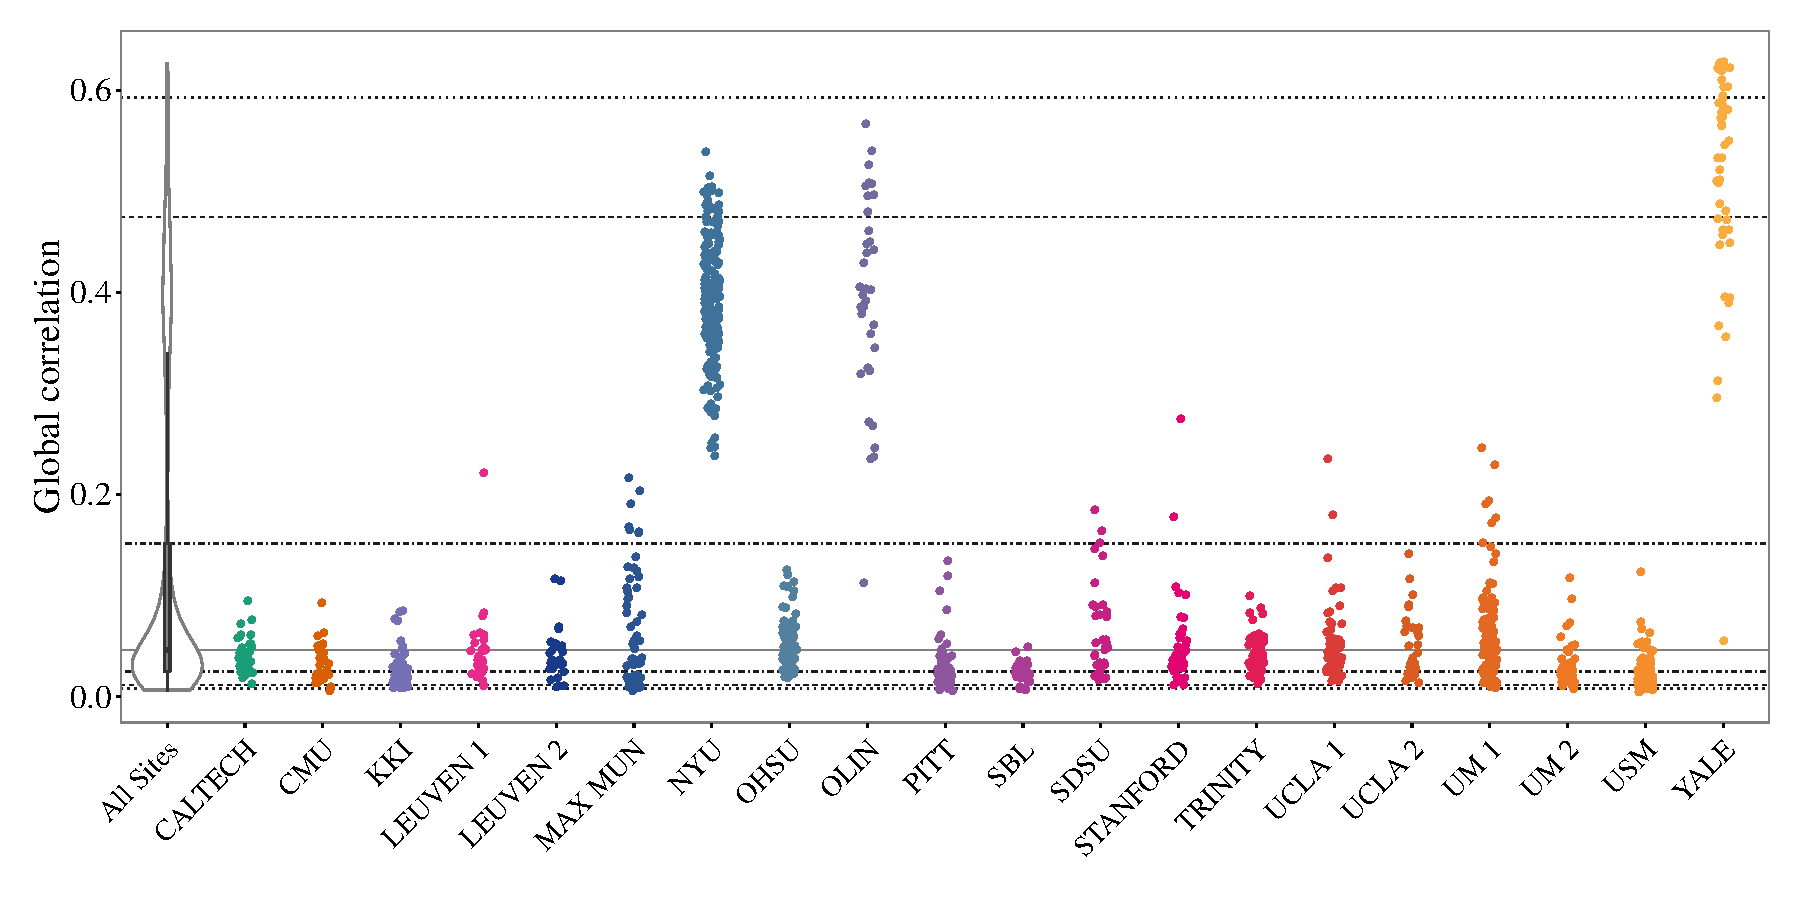
\includegraphics[width=0.9\textwidth]{fig1_ABIDE_Functional_zgcor}
       \caption{GCOR Functional Measure for ABIDE}
     \end{subfigure}
     \begin{subfigure}[b]{0.9\textwidth}
       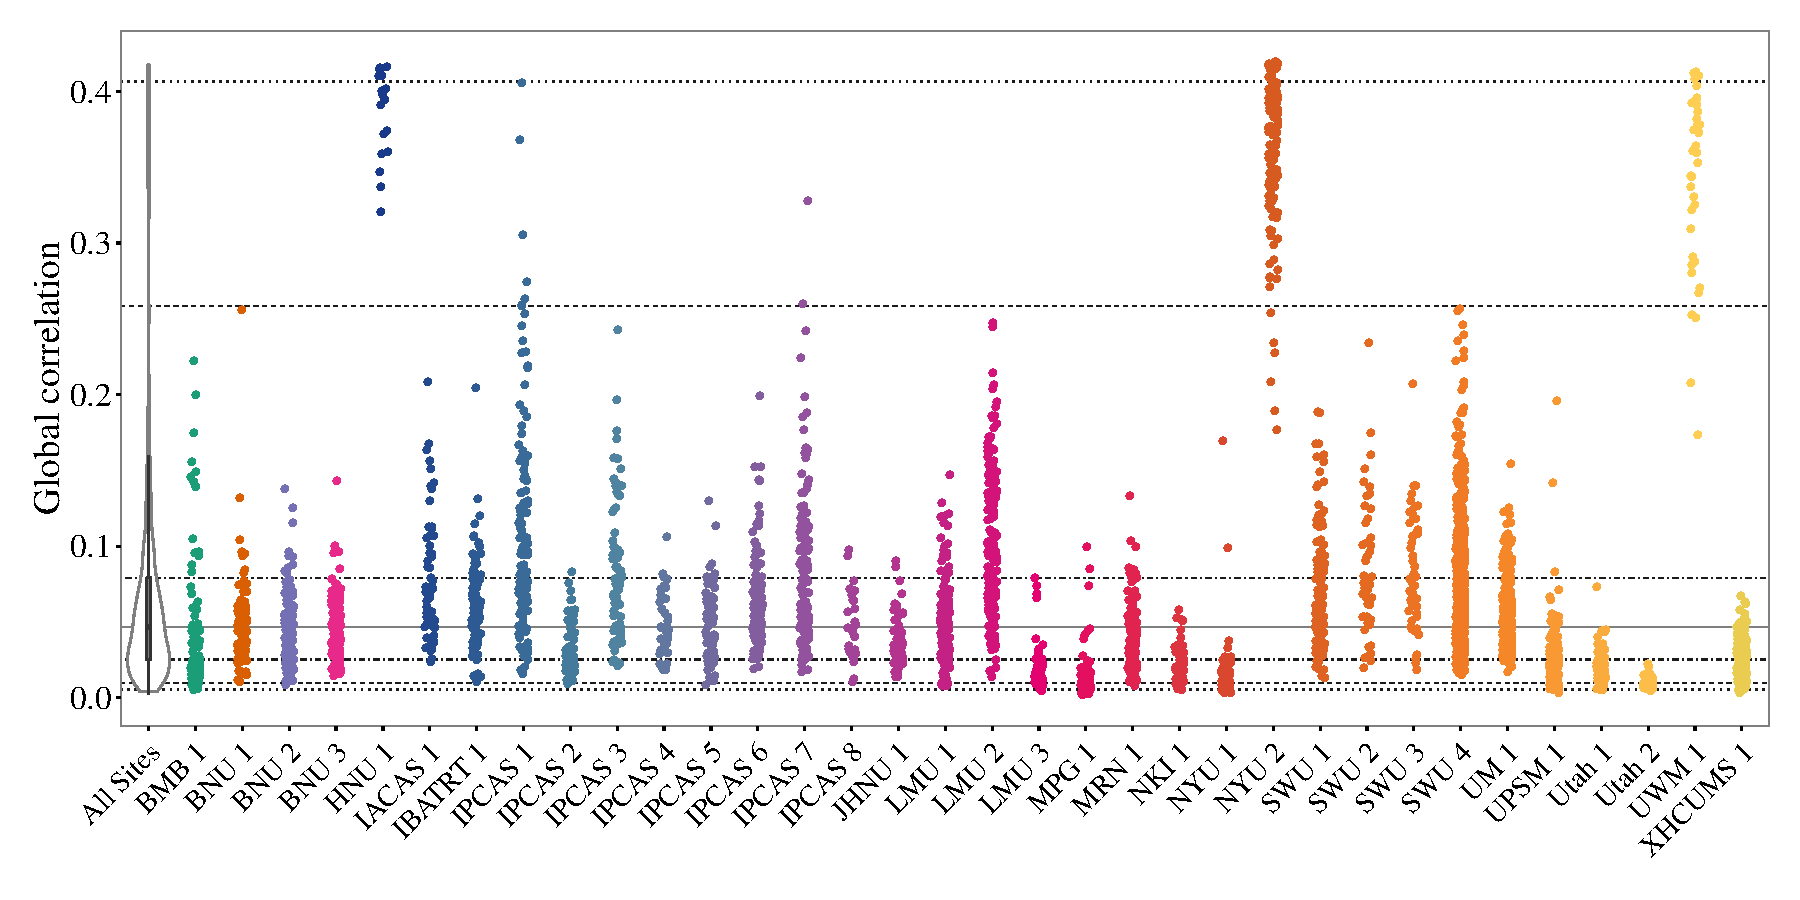
\includegraphics[width=0.9\textwidth]{fig1_CORR_Functional_gcor}
       \caption{GCOR Functional Measure for CoRR}
     \end{subfigure} 
     \caption{Examples of measures and distributions for ABIDE and CoRR}
\end{figure}
\begin{figure}[h]
  \centering
     \begin{subfigure}[b]{0.4\textwidth}
       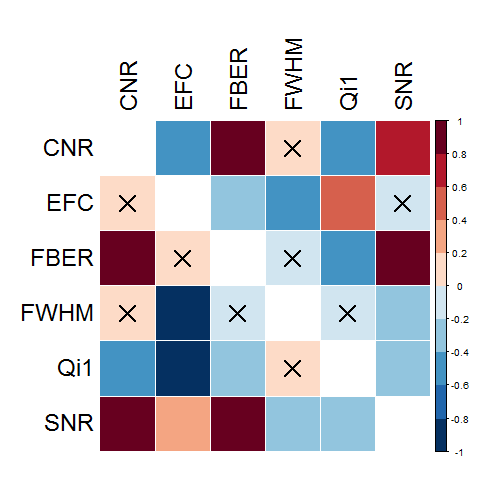
\includegraphics[width=8cm]{fig2_bysite_sig_anat_corrplot}
       \caption{Anatomical measures}
     \end{subfigure}
     \begin{subfigure}[b]{0.4\textwidth}
       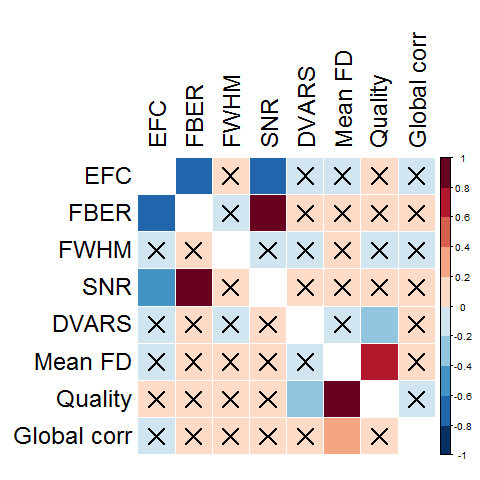
\includegraphics[width=8cm]{fig2_bysite_sig_func_corrplot}
       \caption{Functional measures}
     \end{subfigure} 
     \caption{Correlogram of measures: ABIDE in lower half, CoRR in upper half, X=non-significant}
\end{figure}
\begin{figure}[h]
  \centering
     \begin{subfigure}[b]{0.4\textwidth}
       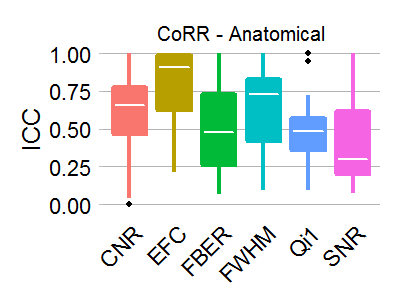
\includegraphics[width=8cm]{fig3_corr_anat_icc_btw}
       \caption{Anatomical measures}
     \end{subfigure}
     \begin{subfigure}[b]{0.4\textwidth}
       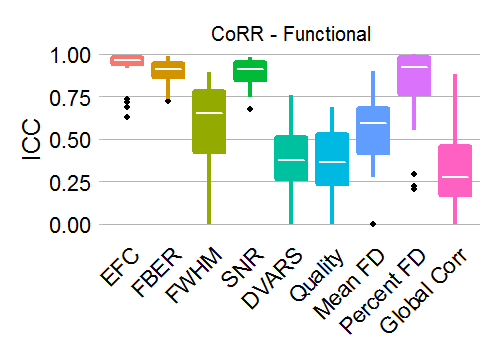
\includegraphics[width=8cm]{fig3_corr_func_icc_btw}
       \caption{Functional measures}
     \end{subfigure} 
     \caption{Test re-test of measures for CoRR}
\end{figure}
\begin{figure}[h]
  \centering
    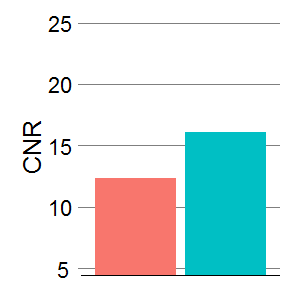
\includegraphics[width=4cm]{fig4_ratings_anat_CNR}
    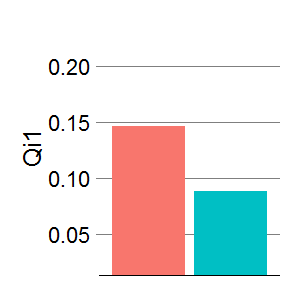
\includegraphics[width=4cm]{fig4_ratings_anat_Qi1}
    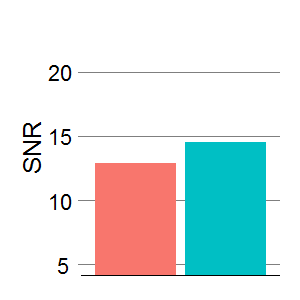
\includegraphics[width=4cm]{fig4_ratings_anat_SNR}
    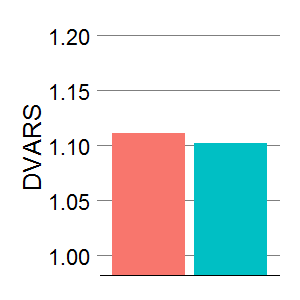
\includegraphics[width=4cm]{fig4_ratings_func_DVARS}
    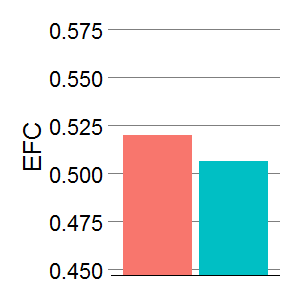
\includegraphics[width=4cm]{fig4_ratings_func_EFC}
    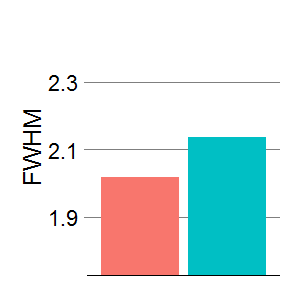
\includegraphics[width=4cm]{fig4_ratings_func_FWHM}
    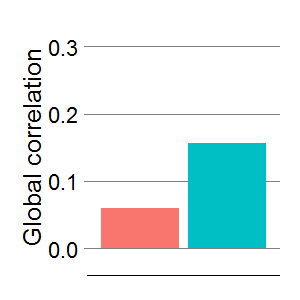
\includegraphics[width=4cm]{fig4_ratings_func_Global_correlation}
    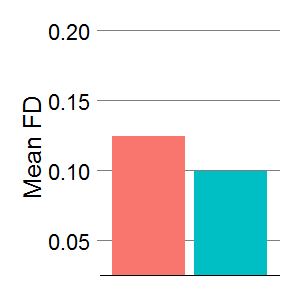
\includegraphics[width=4cm]{fig4_ratings_func_Mean_FD} \\
    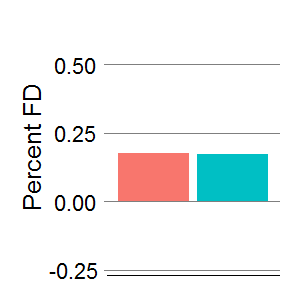
\includegraphics[width=4cm]{fig4_ratings_func_Percent_FD}
    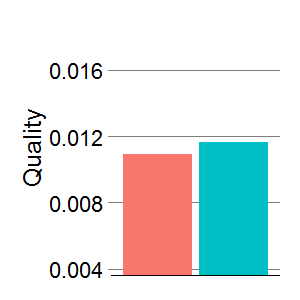
\includegraphics[width=4cm]{fig4_ratings_func_Quality}
  \caption{Most discriminative measures vs. hand assessments}
\end{figure}

%%% Use this if adding the figures directly in the mansucript, if so, please remember to also upload the files when submitting your article
%%% There is no need for adding the file termination, as long as you indicate where the file is saved. In the examples below the files (logo1.jpg and logo2.eps) are in the Frontiers LaTeX folder
%%% If using *.tif files convert them to .jpg or .png

\begin{figure}[h!]
\begin{center}

\includegraphics[width=10cm]{logo1}% This is a *.jpg file
\end{center}
 \textbf{\refstepcounter{figure}\label{fig:01} Figure \arabic{figure}.}{ Enter the caption for your figure here.  Repeat as  necessary for each of your figures }
\end{figure}

%\begin{figure}
%\begin{center}
%
\includegraphics[width=10cm]{logo2}% This is an *.eps file
%\end{center}
%\textbf{\refstepcounter{figure}\label{fig:02} Figure \arabic{figure}.}{ Enter the caption for your figure here.  Repeat as  necessary for each of your figures }
%\end{figure}

%%% If you don't add the figures in the LaTeX files, please upload them when submitting the article.

%%% Frontiers will add the figures at the end of the provisional pdf automatically %%%

%%% The use of LaTeX coding to draw Diagrams/Figures/Structures should be avoided. They should be external callouts including graphics.

\end{document}
